\section{Comments on the Article by Reinhart}

\subsection{Difference between the Radiation Transfer Equation and Reinhart Equation (9)}

\subsubsection{Radiation Transfer Equation}
The radiation transfer equation excluding emission reads:
\begin{align}
	\label{eqn:120}
	\dfrac{d I(\lambda, s)}{ds} = - I(\lambda, s) \sum_i \kappa_i f_i(\lambda)
\end{align}

Integration along the propagation path yields:
\begin{align}
	\dfrac{I(\lambda,s)}{I(\lambda, s = 0)} = \left(1 - \exp\left(-\sum_i \kappa_i f_i(\lambda) s\right)\right)
\end{align}

Integration over a wavelength interval yields:
\begin{align}
	\label{eqn:122}
	\dfrac{I_{abs}}{I_0} = \int_{\Delta \lambda} \left(1 - \exp\left(-\sum_i \kappa_i f_i(\lambda) s\right)\right) d \lambda
\end{align}

\subsubsection{Wavelengths Average Absorption}

Integrating \eqn{eqn:120} over a wavelength interval:
\begin{align}
	\dfrac{d}{ds} \int_{\Delta \lambda} I(\lambda, s) d \lambda = - \sum_i  \int_{\Delta \lambda} I(\lambda, s) \kappa_i f_i(\lambda)  d \lambda
\end{align}
Assuming that the intensity is constant within the integration interval:
\begin{align}
    \dfrac{d I(s)}{ds} &= - \dfrac{I}{\Delta \lambda} \sum_i \kappa_i  \int_{\Delta \lambda}  f_i(\lambda)  d \lambda \\
                    &= - \dfrac{I}{\Delta \lambda} \sum_i \kappa_i(\lambda_i)
\end{align}
Integrating along the propagation path:
\begin{align}
	\dfrac{dI(s)}{I(s)} = - \dfrac{1}{\Delta \lambda} \sum_i \kappa_i ds
\end{align}
yields:
\begin{align}
	\ln \dfrac{I(s)}{I(0)} = - \dfrac{1}{\Delta \lambda} \int_{0}^{s} \sum_i \kappa_i ds
\end{align}
and finally:
\begin{align}
	\label{eqn:128}
	\dfrac{I_{abs}}{I_0} = 1 - \exp\left( - \dfrac{1}{\Delta \lambda} \int_{0}^{s} \sum_i \kappa_i ds \right)
\end{align}

\eqn{eqn:122} and \eqn{eqn:128} result in different values. This is because the assumption of constant intensity 
is in general not valid and that spectrally overlapping lines cannot be treated separatly. 
In the following section a simple is employed to demonstrate this.

\subsubsection{Simple Model}

Two partially overlapping lines with rectangle shaped line shapes:
\begin{figure}[ht]
	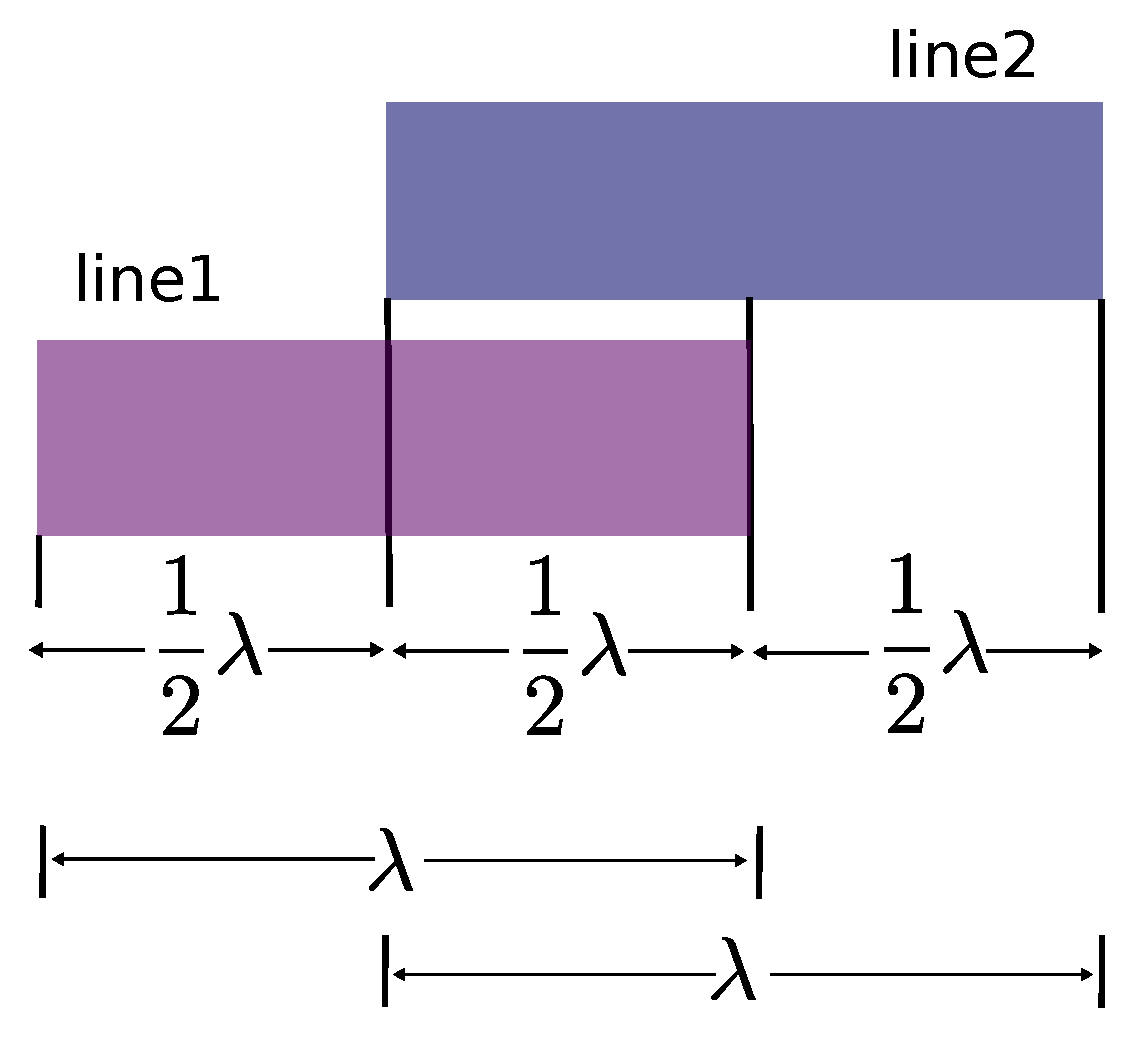
\includegraphics[width=6cm]{figures/overlappinglines2.pdf}
	\caption{Two overlapping lines with rectangle line shape functions}
	\label{fig:overlappinglines}
\end{figure}

Reinhart:
\begin{align}
	\Delta J_1 &= \left(1 - \exp( - \kappa_1 z)\right) \Delta \lambda \\
	\Delta J_2 &= \left(1 - \exp( - \kappa_2 z)\right) \Delta \lambda 
\end{align}
\begin{align}
	A = \dfrac{\Delta J_1 + \Delta J_2}{\Delta \lambda} = \left(1 - \exp( - \kappa_1 z)\right) + \left(1 - \exp( - \kappa_2 z)\right)
\end{align}
Radiation transfer solution :
\begin{align}
	\Delta I_1 &= \left(1 - \exp( - \kappa_1 z)\right) \dfrac{\Delta \lambda}{2} \\
	\Delta I_2 &=  \left(1 - \exp( - \kappa_2 z)\right) \dfrac{\Delta \lambda}{2} \\
	\Delta I_{12} &= \left(1 - \exp( - \kappa_1 z - \kappa_2 z)\right) \dfrac{\Delta \lambda}{2}
\end{align}
\begin{align}
	B = \dfrac{\Delta I_1 + \Delta I_2 + \Delta I_{12}}{I_0 \Delta \lambda} =
			& \dfrac{1}{2} \left(1 - \exp( - \kappa_1 z)\right) +  \\
			& \dfrac{1}{2} \left(1 - \exp( - \kappa_2 z)\right) + \\ 
			& \dfrac{1}{2} \left(1 - \exp( - \kappa_1 z - \kappa_2 z)\right) 
\end{align}
The difference is:
\begin{align}
	2(A - B) &= \left(1 - \exp( - \kappa_1 z)\right) + \left(1 - \exp( - \kappa_2 z)\right) -
	\left(1 - \exp( - \kappa_1 z - \kappa_2 z\right) \\
	         &= 1  + \exp(- \kappa_1 z - \kappa_2 z) - \exp( - \kappa_1 z) - \exp( - \kappa_2 z)
\end{align}
In case of $\kappa_1 \gg 1$ and $\kappa_2 \gg 1$ this yields: 
\begin{align}
	(\Delta J_1 + \Delta J_2) - (\Delta I_1 + \Delta I_2 + \Delta I_{12})=
	I_0 \dfrac{\Delta \lambda}{2}
\end{align}
That means the absorption of the overlapping region is counted twice.